\chapter{Opis projektnog zadatka}
		
		\textbf{\textit{dio 1. revizije}}\\

		Znanstvena udruga “Pametna ekipa” organizira konferenciju na kojoj će sudionici prezentirati svoje radove. Cilj ovog projekta je razviti učinkovit informacijski sustav koji će podržati istovremeni rad više korisnika i ovisno o njihovoj ulozi omogućiti im različite funkcionalnosti. Sudionicima treba omogućiti prijavu na konferenciju i predaju rada s kojim žele sudjelovati, recenzentima da recenziraju zaprimljene radove sudionika, administratoru definiranje upitnika za prijavu i upravljanje sadržajem na samoj web aplikaciji, a predsjedavajućem konferencije da odobrava recenzente te općenito nadgleda podatke sudionika i njihove radove. Dodatno, administrator na web aplikaciji može vidjeti informacije o trenutnoj epidemiološkoj situaciji u državama iz kojih ima prijavljenih sudionika te po potrebi učiniti radove javno dostupnima.
		\newline
		\newline

		Prilikom pokretanja sustava, neregistriranom odnosno neprijavljenom korisniku prikazuje se naslovnica na kojoj se nalazi statičan sadržaj te gumb koji vodi do stranice za registraciju/prijavu. Na vrhu svake stranice  je postavljena traka koja korisniku omogućuje brzo preusmjeravanje na određene stranice: naslovnica, pristup radovima, stranica s kontaktima, te stranica za prijavu u sustav ili profil korisnika ako je korisnik već prijavljen. U slučaju pogoršanja epidemiološke situacije svi će prijavljeni korisnici imati pristup svim odobrenim radovima, a do tada pristup svim radovima imaju samo administrator i predsjedavajući konferencije. Statični sadržaj na početnoj stranici odnosi se na informacije o konferenciji. Na naslovnici se nalazi i dinamičan okvir koji prikazuje sliku i naslov. Okvir može mijenjati sliku korisnikovim klikom na strelicu. Pri ulasku na samu naslovnicu, ukoliko korisnik nije prijavljen, u dinamičnom se okviru pojavljuje veliki gumb "\textit{Registracija}" koji korisnika preusmjerava na registraciju u sustav. 
		\newline
		\newline
		Na stranici za prijavu nalazi se okvir u koji već registrirani korisnici unose korisničko ime i lozinku, a ispod se nalazi gumb koji preusmjerava neregistrirane korisnike na formu za registraciju. Također se ispod okvira nalazi i gumb "\textit{Zaboravljena lozinka}" koji korisniku omogućava slanje nove lozinke na e-mail adresu koju unese. Na stranici za registraciju, odnosno prijavu na konferenciju, postoje dvije opcije: \textit{Registriraj se kao sudionik} i \textit{Registriraj se kao recenzent}. Administrator i predsjedavajući konferencije ne vrše registraciju, već postoji jedan unaprijed definiran administrator koji, ako želi, u sustav dodaje druge administratore čije se funkcionalnosti ne razlikuju od "prvog" administratora. Administrator također određuje predsjedavajućeg konferencije kojemu se na e-mail šalju podatci za prijavu u sustav.
		\newline
		\newline
		\indent Pri registraciji sudionika konferencije potrebni su sljedeći podaci:

		\begin{packed_item}

			\item ime
			\item prezime
			\item korisničko ime
			\item adresa e-pošte
			\item matična ustanova (institucija ili poduzeće) i njezina adresa, grad i država

			\item e-mail adresa
			\item matična ustanova (institucija ili poduzeće) i adresa iste - ulica i kućni broj, grad, država
			\item sekcija u kojoj žele sudjelovati/recenzirati radove koju korisnik odabire iz ponuđene liste

			\item potrebno je odabrati prijavljuje li se osoba kao sudionik ili recenzent
			\item sekcija koju korisnik odabire iz ponuđene liste (recenzent bira u kojoj sekciji će recenzirati radove, a sudionik bira kojoj sekciji pripada rad s kojim se prijavljuje za sudjelovanje na konferenciji)
			\item naslov rada (samo za sudionike)

			\item imena i prezimena autora rada (samo za sudionike)
			\item adresa e-pošte autora kojeg korisnik označi kao osobu za kontakt (samo za sudionike)

		
		\end{packed_item}
	
		U slučaju da neki od podataka nije upisan, sustav javlja kako nisu svi podaci uneseni i traži od korisnika da ih unese ukoliko se želi registrirati. Također se vrši provjera postoji li već u bazi podataka rad istog naslova i autora. Nakon izvršene registracije, ovisno o tome koju ulogu je korisnik odabrao (sudionik ili recenzent) dobit će određena prava koja su objašnjena u nastavku. Korisnik na unesenu adresu e-pošte prima poruku o uspješnoj prijavi, te se u poruci nalazi lozinka koja je potrebna za prijavu u sustav te link na koji mora kliknuti kako bi potvrdio uspješnu registraciju. Sudionici konferencije bi trebali učitati svoj rad u sustav do datuma roka za prijavu na konferenciju koji je javno dostupan.
		\newline
		\newline
		\indent Svaki registrirani korisnik, bez obzira na razinu ovlasti, može pregledavati vlastite korisničke podatke i mijenjati ih po potrebi.
		\newline
		\newline
		Postoje četiri vrste registriranih korisnika:
		\begin{packed_item}
			
			\item administrator
			\item predsjedavajući konferencije
			\item recenzent
			\item sudionik konferencije
			
		\end{packed_item}
	

		\underline{\textit{Administrator}} sustava ima najveću razinu ovlasti. Prilikom samog pokretanja sustava, postoji jedan unaprijed definiran administrator koji, ako želi, u sustav dodaje druge administratore te određuje predsjedavajućeg konferencije. Administrator može mijenjati statički sadržaj na naslovnici, unosi podatke o konferenciji, primjerice definira rok prijave na konferenciju i sekcije u kojima sudionici mogu sudjelovati te definira upitnik za prijavu na konferenciju. U slučaju pogoršane epidemiološke situacije, administrator može dio ili sve radove učiniti javno dostupnima te o tome obavijestiti pojedine (ili sve) sudionike konferencije.
		\newline
		\newline
		\indent \underline{\textit{Predsjedavajući konferencije}} ima glavnu ulogu odobravanja recenzenata. Osim svojih podataka, on također ima uvid u osobne podatke svih sudionika i recenzenata, te ih po potrebi može mijenjati. Također ima mogućnost preuzimanja radova svih sudionika na vlastito računalo. Isto tako, ukoliko se ukaže potreba, može poslati e-poštu pojedinačnim korisnicima ili ga pak poslati svima koji sudjeluju na konferenciji. 
		\newline
		\newline
		\indent \underline{\textit{Recenzent}} je osoba koja recenzira odnosno kontrolira radove sudionika. Svaki rad pregledava samo jedan recenzent, a svaki recenzent može pregledati više radova iz sekcije koju odabere pri prijavi i samo iz te sekcije. Pregledavanjem i recenziranjem radova recenzent odobrava sudjelovanje sudionika na konferenciji. Radove može pregledavati \textit{online} ili ih može preuzeti na računalo i pregledavati. 

		
		Nakon pregleda pojedinog rada, recenzent ima sljedeće mogućnosti:
		
		\begin{enumerate}
			
			\item prihvaćanje rada bez potrebnih izmjena i/ili dopuna rada
			\item prihvaćanje rada, ali sudionik prije finalne predaje mora napraviti manje dorade koje recenzent ne mora provjeriti
			\item prihvaćanje rada, ali uz potrebne značajne izmjene rada o kojima, nakon izvršenja, sudionik mora obavijestiti recenzenta radi njihove provjere
			\item potpuno odbijanje rada uz obrazloženje
			
		\end{enumerate}

		\indent \underline{\textit{Sudionik}} ima najmanju razinu ovlasti - on jedino ima mogućnost pregledavanja i izmjene osobnih podataka te učitavanje radova u sustav. Za njega je glavna svrha sustava upravo prijava na konferenciju i učitavanje rada s kojim želi sudjelovati. Nakon prijave i učitavanja rada u sustav, korisnik ima mogućnost prijaviti još svojih radova.
		\newline
		\newline
		\indent Na internetu se može pronaći mnoštvo primjera sustava za prijavu na različite konferencije. Kod ovakvih sustava važno je da su intuitivni kako bi korisnik lako došao do potrebnih informacija vezanih uz konferenciju i sudjelovanje na njoj. Nije zanemariva ni estetska komponenta web-sučelja jer je jedna od osnovnih svrha ove programske potpore privući potencijalne sudionike, a možda i sponzore. U nastavku se nalaze rješenja koja su služila kao referenca u osmišljavanju sustava.
		\newline
		\newline
		
		\begin{figure}[H]
			\begin{minipage}[t]{0.4\textwidth}
				
\includegraphics[width=\linewidth]{slike/frontpage_example1}
				\caption{\href{https://rstconf.org/}{Primjer rješenja 1.}} \label{fig:frontpage_example1}
			\end{minipage}
			\hspace*{\fill}
			\begin{minipage}[t]{0.4\textwidth}
				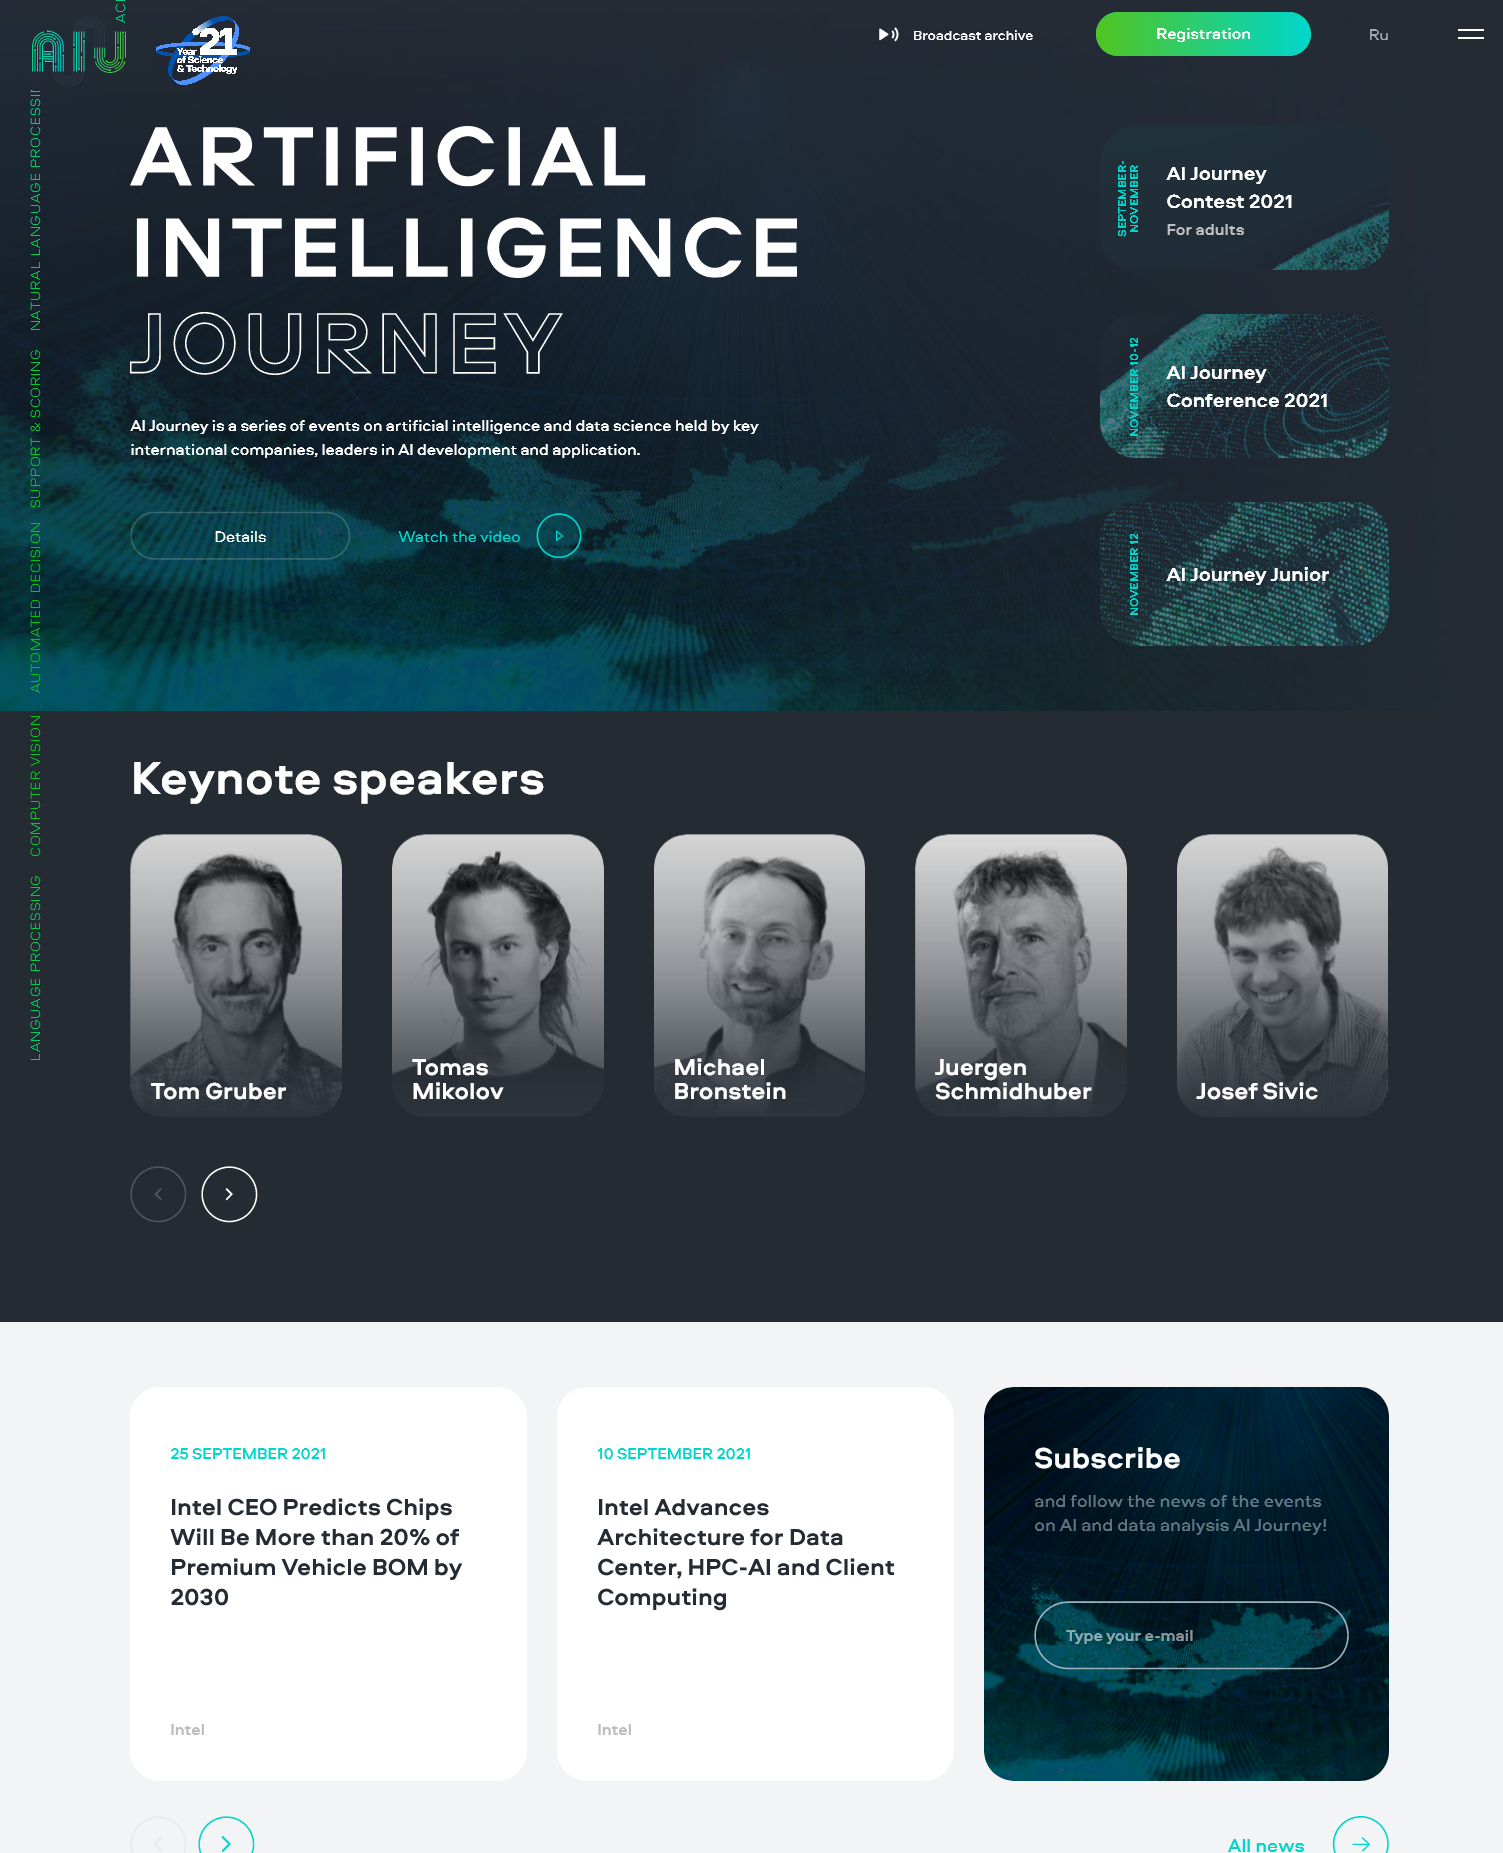
\includegraphics[width=\linewidth]{slike/frontpage_example2}
				\caption{\href{https://ai-journey.ru/en}{Primjer rješenja 2.}} \label{fig:frontpage_example2}
			\end{minipage}
		\end{figure}
		
		\begin{figure}[H]
			\begin{minipage}[t]{0.4\textwidth}
				
\includegraphics[width=\linewidth]{slike/frontpage_example3}
				\caption{\href{http://fof.oac.uncor.edu/2022/}{Primjer rješenja 3.}} \label{fig:frontpage_example3}
			\end{minipage}
			\hspace*{\fill}
			\begin{minipage}[t]{0.4\textwidth}
				
\includegraphics[width=\linewidth]{slike/frontpage_example4}
				\caption{\href{https://www.open-science-conference.eu/}{Primjer rješenja 4.}} \label{fig:frontpage_example4}
			\end{minipage}
		\end{figure}
		
		
		\begin{figure}[H]
			\begin{minipage}[t]{0.4\textwidth}
				
\includegraphics[width=\linewidth]{slike/frontpage_example5}
				\caption{\href{https://gwpaw2021.aei.mpg.de/}{Primjer rješenja 5.}} \label{fig:frontpage_example5}
			\end{minipage}
			\hspace*{\fill}
			\begin{minipage}[t]{0.4\textwidth}
				
\includegraphics[width=\linewidth]{slike/frontpage_example6}
				\caption{\href{https://www.saastrannual2022.com//}{Primjer rješenja 6.}} \label{fig:frontpage_example6}
			\end{minipage}
		\end{figure}
		
		U svim primjerima postoji alatna traka koja se nalazi ili na vrhu, ili u sredini stranice (u Primjerima 3. i 5.). Isto tako, na vrhu svakog primjera nalazi se upečatljiva naslovna slika sa velikim naslovom čije se boje i sadržaj uklapaju u temu konferencije. Osim datuma koji je istaknut jače ili slabije na svakoj stranici, Primjeri 1., 4. i 5. također prikazuju i lokaciju održavanja konferencije, odnosno informaciju ako se održava \textit{online}. Poslije naslovne slike, osim u Primjerima 2. i 6., prikazuje se statični sadržaj s informacijama o samoj konferenciji, dok ostala dva primjera također prikazuju statični sadržaj, ali manje detaljan. Svaka stranica ima istaknut gumb koji korisnika usmjerava na registraciju u sustav. Primjeri 2. i 3. imaju tamnu glavnu temu sa svijetlim tekstom, dok preostali primjeri imaju svijetlu temu s tamnim tekstom, što upućuje na važnost kontrasta pozadine i teksta radi lakše čitljivosti. 
			
		\eject
		
	